
\chapter{QuickMap : another NetGen-compatible map browser}

\begin{quote}

{\sl \bf{Note :} QuickMap is developed by Pierre-Yves Lucas as a geographic frontend to NetGen.}

\end{quote}

\label{sec:chapter5bis}

This chapter will present QuickMap, an evolution of the tool presented in chapter \ref{sec:chapter5}
designed to support precise geographic positions and easy map  browsing. 


A movie is available at {\tt http://wsn.univ-brest.fr/QuickMap/} that demonstrates 
the tool in action to describe and control field of sensors,  working
under the control of satellite.

QuickMap has also support for displaying 
buildings or obstacles representations extracted from OpenStreetMap databases. 
The present tools allow to interact with the more common tiles servers. 
An example of such a server is OpenStreetMap reachable at http://tile.openstreetmap.org\footnote{See the 
explanations about access agreement, keeping in mind that the present software is 
a reserch investigation, and not a production application}.


\begin{figure}[hbtp]
\begin{center}
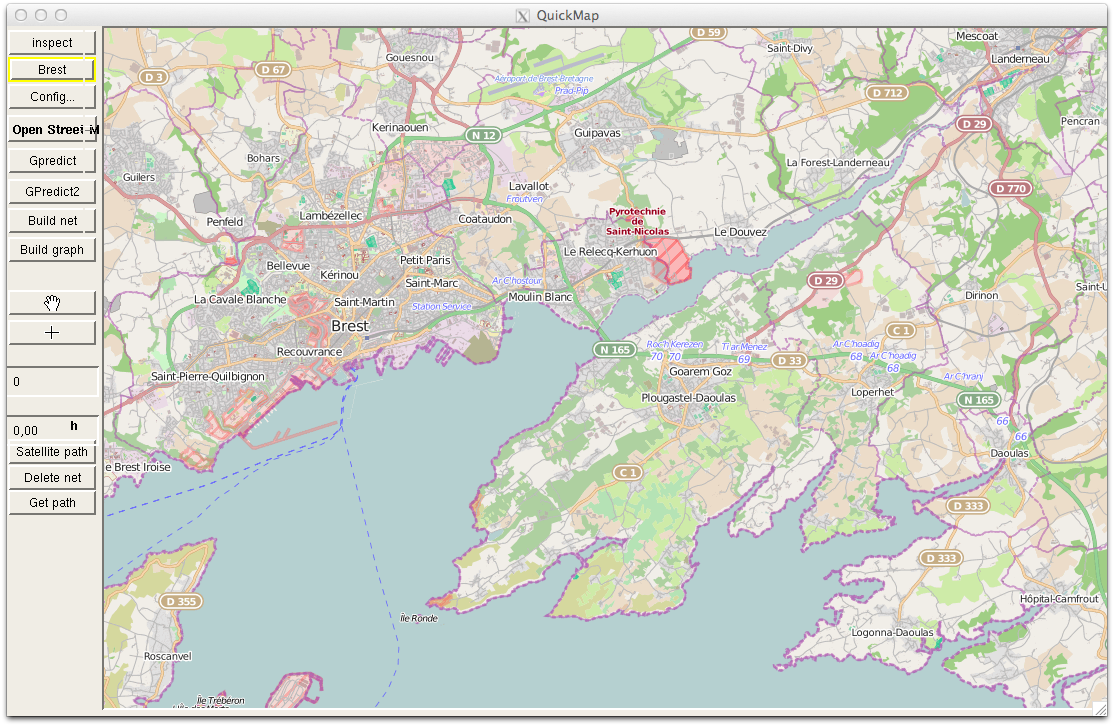
\includegraphics[width=10cm]{QuickMapSatBrest.png}
\caption{Initial view on QuickMap version for satelite control,
pointng to default Brest location. The user interface allows to move directly maps using
the hand cursor. The sensor wheel controls depth in the map system, here OpenStreetMap.}
\label{fig:initialQuickMapBrest}
\end{center}
\end{figure}

The map browser is a tool allowing to display various kind of maps and to represent 
locations of interest such as sensors set in the country. 
As this tool is developped on the same platform as NetGen, the procedures described 
in chapter \ref{sec:chapter1} will apply to access the software: 
\begin{itemize}
\item start a fresh image and ensure that the NetGen package is loaded with one of the last version,
\item open the store dialog from VisualWorks main window menu ba,
\item select QuickMap package ,
\item select last version, and type load from the pop-up menu
\end{itemize}

Once the package is loaded, launching is achieved from the Tools menu, with a number of variants
available (figure \ref{fig:toolsMenu} ).

\begin{figure}[hbtp]
\begin{center}
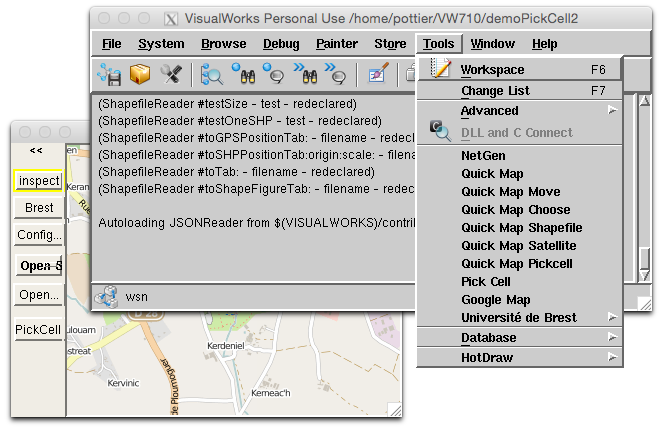
\includegraphics[width=10cm]{toolsMenu.png}
\caption{Tools menu after loading QuickMap, select one of the interfaces from here.}
\label{fig:toolsMenu}
\end{center}
\end{figure}


\section{Short presentation}

Figure 
\ref{fig:initialQuickMapBrest} shows a view on a QuickMap windowi with a number
of control button on the left, and map display on the right.


\begin{figure}[hbtp]
\begin{center}
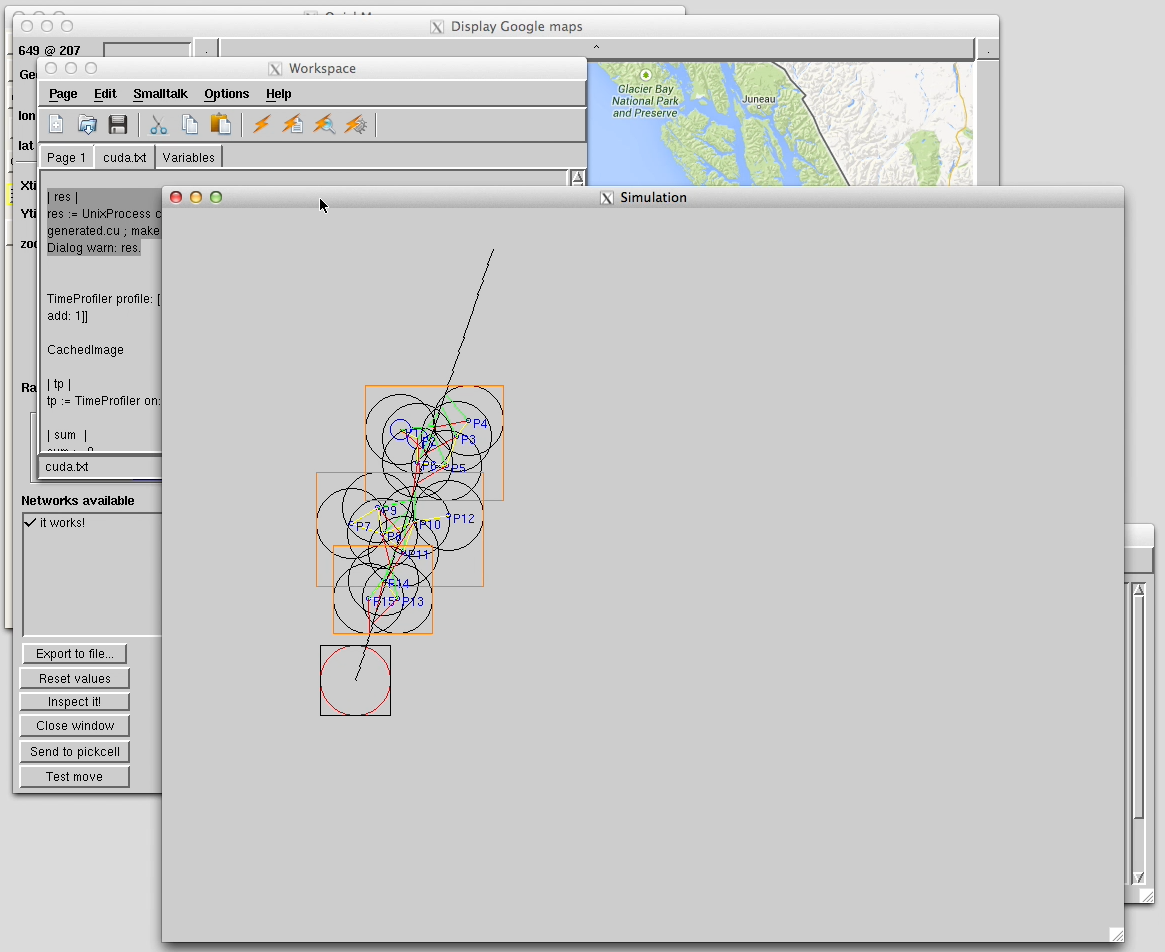
\includegraphics[width=12cm]{QuickMapDemo.png} 
\caption{End of simulation, showing the satellite path and subsystem bounding boxes.}
\label{fig:QuickMapDemo}
\end{center} 
\end{figure}

The movie proposed at  {\tt http://wsn.univ-brest.fr/QuickMap/} is a sequence representing 
the current tool status (figure \ref{fig:QuickMapDemo}):

\begin{description}
\item  [Moving the map ]: shows horizontal and vertical moves on an OpenStreetMap map system. 
\item [Launching GPredict  ]: external software that allows to select satellite and pipe informations to QuickMap. 
\item [Following Satellite ]: these values are collected and presented on QuickMap, the red ball figures the selected satellite. 
\item [Specification of a sensor field]: some sensors are positioned in front of the satellite path.
\item [Building networks ]: build button ask computation of edges representing communication links establishment and disconnection.
\item [Network synthesis ]: using the old version of the browser, the communication ranges can be modified, then the problem is passed to NetGen for simulatioon (CUDA).
\item [System simulation ]:  satellite and sensors work together, synchronously. The distributed program start at the same step
on the ground and in the air. Bounding box for controlled sensor systems are computed and displayed.
\end{description}

\section{Building sensor fields}

Movie available at  {\tt http://wsn.univ-brest.fr/QuickMap/}, select some version of {\tt fieldOfSensorsSpec.mov}.

The flow is as follows:

\begin{description}
\item [Launch QuickMap, option satellite] : then navigate to a zone where the field must be installed,
\item [Select a zone ]: select the crosshair cursor, type the number of sensors in the input field on the left, and clic top left, then bottom right.
\item [Following Satellite ]: these values are collected and presented on QuickMap, the red ball figures the selected satellite.
\item [Build graph ]:  displays a net with a default range.
\item [Build net ]:  open a GMap window, from which you can :
\begin{enumerate}
\item refresh map to your sensor field
\item change the radio range
\item draw resulting net (see Figure \ref{fig:enezEussa})
\end{enumerate}
\item [Generate abstract specification ]: open a NetGen window from the general Tool menu, then press build simulations from GMap
\item [Save simulators ]: change the network name to something like "enezEussa", or "Sahara", select generation options, and accept-and-save from the pop-up menu.
\item [Observe results ]:  files are in the local Generated directory, Occam, Cuda, or graphviz formats.
\end{description}



\begin{figure}[hbtp]
\begin{center}
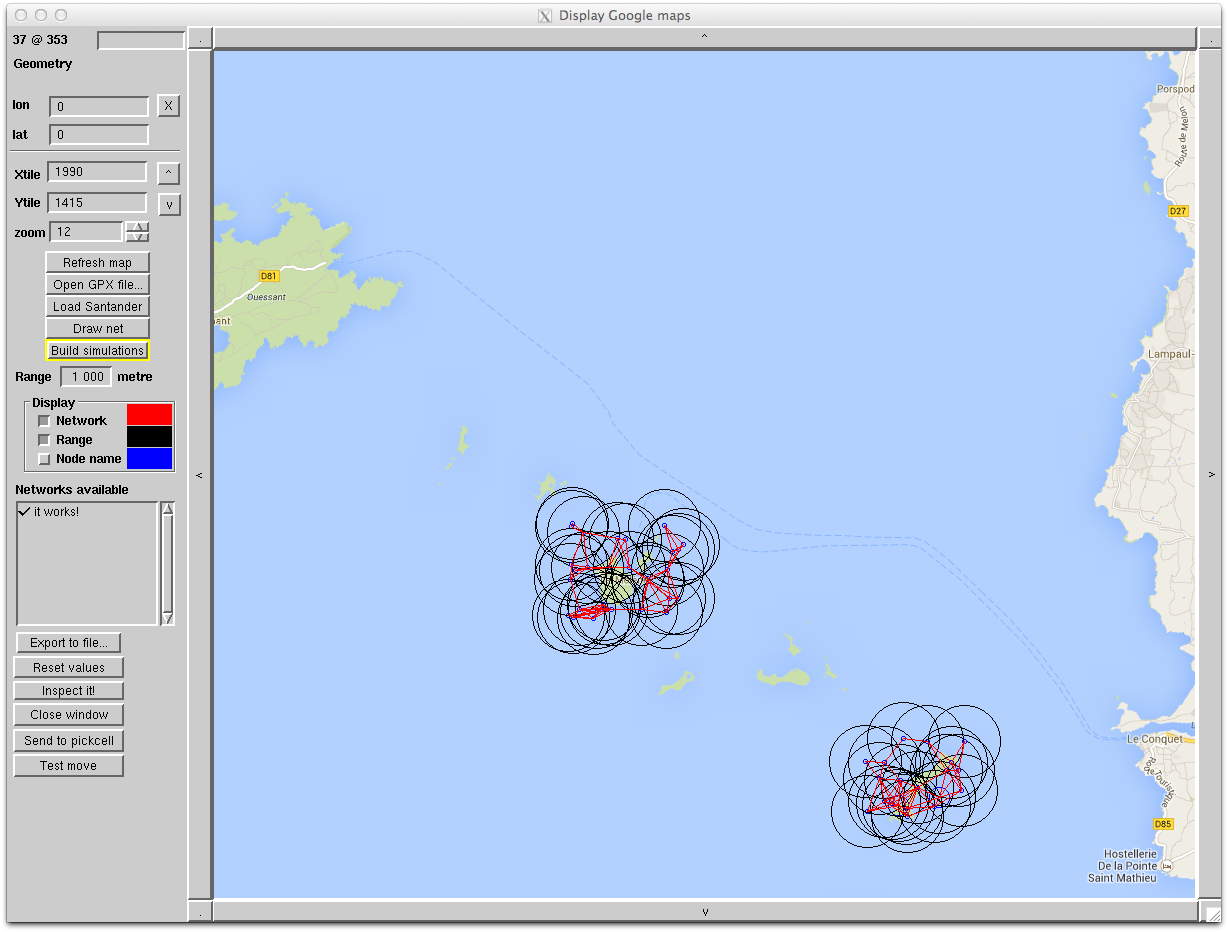
\includegraphics[width=10cm]{MolenePlus.png}
\caption{Random sensor field over Iroise islands, 1Km radio range, two fields of different sizes. 50 random positions.
Simply press + as many time as necessary to obtain several rectangle, and thus, several fields. }
\label{fig:enezEussa}
\end{center}
\end{figure}
